\documentclass{book}

\usepackage[utf8]{inputenc}
\usepackage[spanish]{babel}
\usepackage{graphicx}
\usepackage{amsmath}
\usepackage{amssymb}
\usepackage{wrapfig}
\usepackage{vmargin}


\author{Armando Rivera}
\title{Machine Learning}
%\setpapersize{A4}

\begin{document}
\maketitle
\renewcommand{\tablename}{Tabla}
\renewcommand{\listtablename}{Índice de tablas}
\tableofcontents
\listoffigures
\listoftables
\chapter{Introducción}
El aprendizaje automático es una
de las nuevas tecnologías más emocionantes. Cada vez que usas un buscador web como Google o Bing para hacer una
búsqueda en internet, una de las razones por las que funciona tan bien es porque
un algoritmo de aprendizaje, implementado por Google o Microsoft, ya aprendió a clasificar las
páginas web. Cada vez que usas Facebook o o que la aplicación de fotos de Apple
reconoce las fotos de tus amigos, eso es aprendizaje automático. \\\\Cada vez que lees
tu correo electrónico o que tu filtro de spam te salva de tener toneladas de correo basura,
eso también es un algoritmo de aprendizaje.\\¿Por qué
predomina el aprendizaje automático hoy en día? Resulta que el aprendizaje automático es un
campo que nació a partir de la IA o inteligencia artificial. Queríamos
construir máquinas inteligentes y resulta que hay pocas cosas básicas que
podemos programar para que haga una máquina como encontrar la ruta más corta de A a B.
Pero en gran medida no sabíamos cómo hacer programas de IA para hacer cosas
más interesantes como buscar en la web, etiquetar fotos o antispam. Se comprendió
que la única forma de hacer estas cosas era que una máquina aprendiera
a hacerlas por sí misma. Así que el aprendizaje automático se desarrolló como una nueva capacidad
para las computadoras y hoy está en muchos sectores de industria y ciencia básica.\\\\Veamos otros ejemplos de aprendizaje automático. Existe la minería de datos.
Una de las razones por las que el aprendizaje automático se ha difundido es el crecimiento de la web y
de la automatización, es decir, que ahora tenemos más datos que
nunca. Por ejemplo, hoy en día muchas empresas en Silicon Valley recolectan datos de
clics, también llamados datos de tráfico, y tratan de usar algoritmos de aprendizaje
electrónico para explorar estos datos y entender mejor a los usuarios y darles
mejor servicio. Actualmente es un gran segmento de Silicon Valley. Expedientes
médicos. Ahora con la llegada de la automatización, tenemos expedientes médicos electrónicos, entonces si
convertimos los expedientes médicos en conocimientos médicos, empezaremos a entender mejor
la enfermedad. Biología informática. También con la automatización los biólogos
recolectan muchos datos sobre la secuencia genética, secuencias de ADN, etc.
y los algoritmos de aprendizaje automático nos ayudan a entender mejor el genoma
humano y qué significa ser humano. También en ingeniería, en todos las áreas de
ingeniería, tenemos conjuntos de datos cada vez más y más grandes, que
tratamos de entender mediante algoritmos de aprendizaje.\\\\ Actualmente, la mayoría del procesamiento de
lenguaje natural y de visión por computadora aplica aprendizaje automático. Los algoritmos de
aprendizaje se utilizan mucho en los programas de autopersonalización. Cada vez que entras a
Amazon, Netflix o iTunes Genius y te recomienda películas, productos y música,
eso también es un algoritmo de aprendizaje. Si lo piensas, tienen millones de usuarios;
no hay forma de crear un millón de programas distintos para esos usuarios.
La única manera de que el software genere estas recomendaciones personalizadas es
que pueda aprender por sí mismo tus preferencias. Por último, los algoritmos
de aprendizaje se usan hoy en día para entender el aprendizaje humano
y para entender el cerebro.\\ Hace algunos meses, un estudiante me mostró un artículo.
\section{Qué es Machine Learning}
Entre los practicantes del aprendizaje
automático no existe una definición bien aceptada sobre lo que es y lo que no es aprendizaje automático.\\
Pero vamos a ver un par de ejemplos sobre las maneras en
que la gente ha intentado definirlo. Esta es la definición sobre qué es aprendizaje automático para
\textbf{Arthur Samuel}. Definió el aprendizaje automático como \textit{el campo de estudio que le da a los ordenadores la habilidad de aprender algo sobre lo que no han sido explícitamente programados.}\\\\ La fama de Samuel se remonta a la década
de 1950, cuando escribió un programa para jugar a las damas.
Y lo asombroso sobre este programa que juega a las damas era que el propio Arthur Samuel
no era un buen jugador de damas. Pero lo que él hizo fue, tener un programa para jugar
decenas de miles de partidas contra si mismo. Y observando que tipo de posiciones en el tablero
tienden a conducir a la victoria y que tipo de posiciones en el tablero tienden a
perder.\\ El programa de juego de damas aprende con el tiempo que posiciones son buenas
en el tablero y cuales son malas posiciones. Y, finalmente, aprender a jugar
a las damas mejor de lo que el propio Arthur Samuel era capaz. Esto fue un resultado notable.
Aunque el propio Samuel resultó no ser un jugador de damas muy bueno. Pero debido a que el
ordenador tiene la paciencia para jugar decenas de miles de partidas contra él mismo. Ningún
humano tiene la paciencia para jugar esa cantidad de partidas. De esta manera el ordenador fue capaz de
obtener una gran experiencia jugando a las damas que, finalmente llegó a ser
mejor jugador que el propio Arthur Samuel.\\\\ Esta es una definición
un tanto informal, y algo más antigua. Aquí está una definición un poco más reciente de\textbf{ Tom
Mitchell}, Entonces Tom define el aprendiza automático
diciendo que, \textit{Un programa de ordenador se dice que aprende de la experiencia\textbf{ E}, con respecto a \textbf{T}, y alguna
medida de rendimiento\textbf{ P}. Y si esta actuación en\textbf{ T}, medida por \textbf{P} mejora
la experiencia\textbf{ E}.}\\\\
Para el ejemplo de jugadores de damas, la experiencia \textbf{E}, será la
experiencia de tener el programa jugando decenas de miles de partidas reiteradas contra él mismo.
La tarea \textbf{T}, será la tarea de jugar partidas. Y la medida de mejora \textbf{P},
será la probabilidad que lo haga ganar la siguiente partida de damas contra
un nuevo oponente.
\section{Aprendizaje Supervisado}
Supongamos que quieres
predecir precios de casas. Y digamos que trazas un conjunto de datos y se ve
así. En la figura \ref{fig:Ej1} tenemos en el eje horizontal, el tamaño de distintas casas en pies cuadrados,
y en el eje vertical, el precio de distintas casas en miles de dólares.
Entonces, con estos datos, digamos que tienes un amigo que tiene una casa de 750
pies cuadrados y desea venderla y quiere saber cuánto dinero puede
obtener por ella. Entonces, ¿cómo puede ayudarte un algoritmo de aprendizaje?\\\\ Algo que podría hacer
el algoritmo de aprendizaje es trazar una línea recta a través de los datos o insertar
una línea recta en los datos y, con base en eso, resulta que tal vez la casa pueda venderse
en aproximadamente \$150,000. Pero tal vez este no es el único algoritmo de aprendizaje que puedes
usar. Puede haber uno mejor. Por ejemplo, en lugar de trazar una línea
recta en los datos, podríamos decidir que es mejor insertar una función
cuadrática o un polinomio de segundo grado a estos datos. Y si haces eso y haces una
predicción aquí, entonces resulta que tal vez puede vender la casa en casi
\$200,000. \\\\
el término aprendizaje supervisado se refiere al hecho de que le dimos al algoritmo un conjunto de datos
donde se daban las ``respuestas correctas". Es decir, le dimos un conjunto de datos
de casas en los que para cada ejemplo del conjunto de datos, se dijo cuál era el
precio correcto, el precio real al que se vendió esa casa y la tarea del
algoritmo sólo fue generar más ``respuestas correctas" como para esta
casa nueva que tu amigo está queriendo vender. Para definir un poco más
la terminología, esto también se denomina un problema de regresión y con esto
quiero decir que queremos predecir un resultado de valor continuo. Es decir, el precio.
Así que, técnicamente, creo que puede redondearse el precio al centavo más cercano. Tal vez
los precios en realidad son valores discretos, pero en general pensamos en el precio de una casa
como un número real, un valor escalar, un número de valor continuo, y el término
regresión se refiere al hecho de que tratamos de predecir el tipo de atributo valuado
de forma continua.\\\\
\begin{figure}
	\centering
	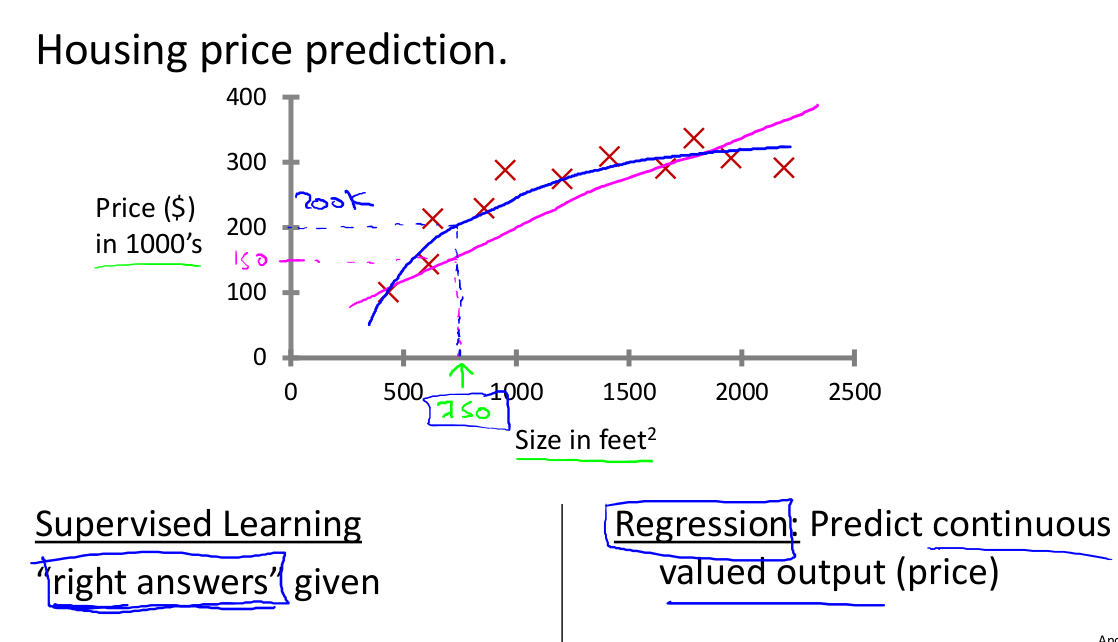
\includegraphics[scale=0.35]{img/Ej1}
	\caption{Ejemplo de aprendizaje supervisado}
	\label{fig:Ej1}
\end{figure}

Digamos que quieres revisar
expediente médicos y tratar de predecir cáncer de mama como maligno o benigno. \\Un tumor maligno es un
tumor dañino y peligroso y un tumor benigno es un tumor inofensivo.
Veamos  en la Figura \ref{fig:Ej2} un conjunto de datos recolectados y supongamos
que en estos datos, en el eje horizontal tienes el tamaño del tumor y
en el vertical, sí o no, si o no son
ejemplos de tumores, el uno si es maligno o el cero si no es maligno.\\\\ Supongamos que nuestro conjunto de datos se ve así donde vemos algunos tumores de varios 
tamaños que resultaron ser benignos.\\
Por desgracia, también vemos unos tumores malignos. Así que en este ejemplo tengo cinco ejemplos de tumores
benignos que se muestran abajo y cinco de tumores malignos que se muestran con un
valor del eje vertical de uno.\\ Y digamos que tenemos una amiga que lamentablemente tiene un
tumor mamario y supongamos que su tamaño es de aproximadamente del valor mostrado con la flecha magenta en la figura \ref{fig:Ej2}. La
pregunta de aprendizaje automático es: ¿puedes calcular cuál es la probabilidad,
de que un tumor sea maligno versus benigno?\\\\ Para mostrar un poco
de terminología, este es un ejemplo de un problema de clasificación. El término
``clasificación" se refiere al hecho de que intentamos predecir un resultado
de valor discreto: cero o uno, maligno o benigno. Y resulta que algunas veces
en problemas de clasificación, puedes tener más de dos valores para dos
posibles valores para el resultado.\\ Como ejemplo concreto tal vez haya tres
tipos de cáncer de mama, por lo que puedes intentar predecir el valor discreto de cero,
uno, dos o tres, en el que cero es benigno. Tumor benigno, es decir sin cáncer. Y uno puede
significar un tipo de cáncer, si tienes tres tipos de cáncer, lo que sea que signifique
el tipo uno. Y dos puede significar un segundo tipo de cáncer y tres pude ser un tercer tipo de
cáncer. Pero esto también sería un problema de clasificación, debido al otro
conjunto de resultados del valor discreto que corresponde a: sin cáncer o cáncer tipo
uno, tipo dos, o cáncer tipo tres.\\\\

\begin{figure}
	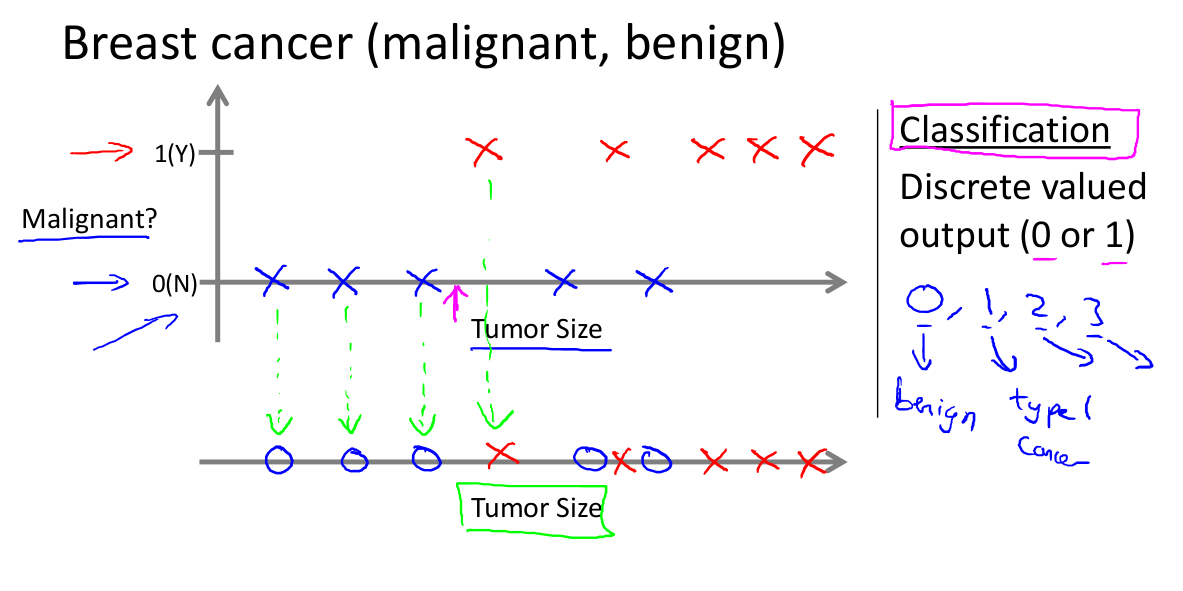
\includegraphics[scale=0.35]{img/Ej2}
	\caption{Ejemplo de clasificación}
	\label{fig:Ej2}
\end{figure}

Existe otra forma de trazar estos datos
en los problemas de clasificación.  Así que si el tamaño del tumor será
el atributo que se usará para predecir si es maligno o benigno, En lugar de dibujar cruces,se dibujarán círculos para los tumores benignos. Y se usarán X para denotar los tumores malignos. Todo lo se hizo fue tomar el conjunto de datos de arriba en la Figura \ref{fig:Ej2} y se dibujaron abajo.\\\\ En este ejemplo sólo usamos una característica o un atributo, principalmente, el tamaño del tumor para predecir si el tumor es maligno o es benigno.\\ \\

Digamos que en lugar de sólo saber el tamaño del tumor, también conocemos la
edad y el tamaño de tumor de los pacientes. En ese caso, tal vez tu conjunto de datos se verá como en la figura \ref{fig:Ej3} y tenemos un conjunto de pacientes cuyos tumores resultaron malignos, como lo indican las cruces.\\

\begin{figure}
	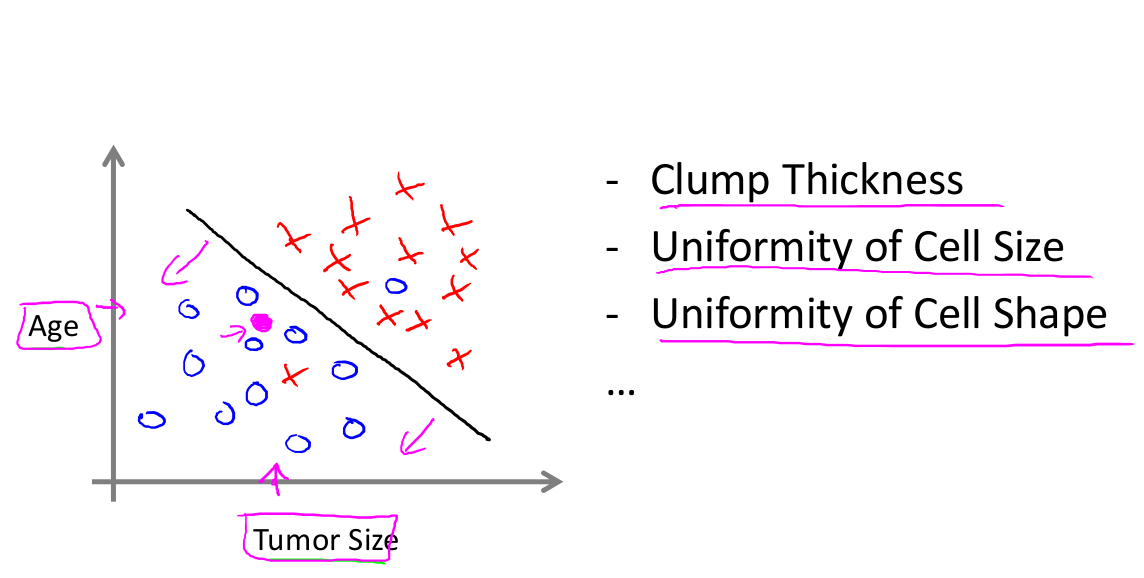
\includegraphics[scale=0.35]{img/Ej3}
	\caption{Problema de clasificación con dos variables}
	\label{fig:Ej3}
\end{figure}

Así que digamos que
tienes un amigo que por desgracia tiene un tumor. Y tal vez, el tamaño del tumor y la edad
están más o menos donde indica el punto color magenta. Con un conjunto de datos como este, lo que puede hacer el
algoritmo de aprendizaje es trazar la línea recta en los datos para tratar de separar los
tumores malignos de los benignos y entonces el algoritmo de aprendizaje puede decidir
trazar la línea recta para separar las dos clases de tumores.
Y con esto, es posible que puedas decidir que es más probable.\\\\En este ejemplo, tuvimos dos características,
la edad del paciente y el tamaño del tumor. En otros problemas de aprendizaje automático
con frecuencia tendremos más características como el grosor de acúmulo del
tumor mamario, uniformidad del tamaño celular del tumor, uniformidad de la forma celular del
tumor, etc., así como otras características. Resulta que para algunos problemas
de aprendizaje, lo que realmente no quieres es usar tres o cinco características, sino
usar un número infinito de características, un número infinito de
atributos, de manera que tu algoritmo de aprendizaje tenga muchos atributos o
características o señales para hacer las predicciones. Entonces, ¿cómo manejas un
número infinito de características? ¿Cómo almacenas un número infinito de
cosas en la computadora cuando sabes que se va a llenar la memoria? Resulta
que cuando nos referimos a un algoritmo llamado Máquina de
Soporte Vectorial, habrá un truco matemático genial que permitirá que la computadora maneje
un número infinito de características. \\\\ En el aprendizaje supervisado, cada ejemplo de
nuestro conjunto de datos, nos dice que la ``respuesta correcta" que nos habría gustado,
la predijeron los algoritmos en ese ejemplo. Como el precio de la
casa o si el tumor es maligno o benigno. También hablamos sobre el
problema de regresión. Y regresión significa que nuestro objetivo es predecir
un resultado de valor continuo. Y hablamos sobre el problema de clasificación, donde
el objetivo es predecir el resultado de valor discreto. Solo una pregunta para recapitular:
Supongamos que diriges una empresa y quieres desarrollar algoritmos de aprendizaje
para enfrentar los dos problemas. En el primer problema, tienes un gran inventario de
artículos idénticos. Entonces, imagina que tienes miles de copias de algunos artículos
idénticos para vender y quieres saber cuántos de estos artículos venderás en los
próximos tres meses. En el segundo problema, el problema dos, tendrás muchos
usuarios y querrás diseñar un software para analizar cada una de las
cuentas individuales de tus clientes, cada una de las cuentas de tus clientes; y para cada cuenta
decidirás si la cuenta fue o no hackeada o estuvo en peligro. Entonces, ¿cada uno
de estos problemas debe tratarse como un problema de clasificación o
como un problema de regresión? \\\\ Por problema uno lo trataría como un
problema de regresión, ya que si tuviera miles de artículos, bueno,
probablemente lo trataría como un valor real, como un valor continuo. Y
por lo tanto, trataría el número de artículos que vendo como un valor continuo. Y para el
segundo problema, lo trataría como un problema de clasificación, ya que podría
establecer el valor que quiero predecir con cero para denotar que no se hackeo
la cuenta. Y establecer el valor en uno para denotar una cuenta que sí fue hackeada. Así
como para el cáncer de mama cero es benigno y uno es maligno. Por ello
podría establecerlo en cero o uno dependiendo de si se hackeó y hacer que un
algoritmo trate de predecir cada uno de estos dos valores discretos. Y debido a que existe
un número reducido de valores discretos, entonces lo manejaría como un problema de
clasificación.
\newpage
\section{Aprendizaje no supervisado}
En el aprendizaje no supervisado nos dan el conjunto de datos
y no nos dicen qué
hacer con eso y no nos
dicen cuál es cada punto de datos.
En lugar de eso, nos dicen aquí está el conjunto de datos.
¿Puedes encontrar alguna estructura en los datos?
Con estos datos, un
algoritmo de aprendizaje no supervisado podría decidir
que lo datos están en dos grupos diferentes.
Así que hay un grupo
y un grupo diferente.
A esto se le llama algoritmo de agrupamiento.\\\\
El aprendizaje no supervisado nos sirve para hacer el agrupamiento de datos o clustering, también nos sirve para la reducción de dimensionalidad, por ejemplo si tenemos muchos datos y queremos trabajar únicamente con un sector.
Cluster: Se puede trabajar con segmentación de mercado. Sistemas de recomendación.
Reducir dimensionalidad: Visualización Big data. Descubrimiento de estructuras.
Algoritmos:
k-means: k es el numero de grupos, cada grupo tendrá un centro (Centroide) y alrededor de este centro se ubicaran datos con caracterísicas similares.
\\\\
El aprendizaje no supervisado nos permite abordar problemas con poca o ninguna idea de cómo deberían ser nuestros resultados. Podemos derivar la estructura de datos donde no necesariamente sabemos el efecto de las variables.

Podemos derivar esta estructura agrupando los datos en función de las relaciones entre las variables en los datos.

Con el aprendizaje no supervisado no hay retroalimentación basada en los resultados de la predicción.\\

Ejemplo:\\

Agrupación: tome una colección de 1,000,000 de genes diferentes y encuentre una manera de agrupar automáticamente estos genes en grupos que de alguna manera sean similares o estén relacionados por diferentes variables, como la duración de la vida, la ubicación, los roles, etc.

Sin agrupación: el ``algoritmo de cóctel", le permite encontrar la estructura en un entorno caótico. (es decir, identificar voces individuales y música de una malla de sonidos en un cóctel).

\chapter{Regresión Lineal con una variable}
La regresión lineal predice una salida de valor real basada en un valor de entrada. Discutimos la aplicación de la regresión lineal a la predicción del precio de la vivienda, presentamos la noción de una función de costo e introducimos el método de pendiente de gradiente para el aprendizaje.
\section{Modelo y función de costo}
\subsection{Modelo y representación}
En la figura \ref{Fig:MR1} tenemos datos de los precios de distintas casas con sus repectivas áreas. Supongamos que queremos obtener un dato que no está en la gráfica, por ejemplo, queremos comprar una casa de 1250 $(feet^2)$ con una aproximación sabremos que nos costará \$220k. 
La regresión lineal nos permite predecir un valor a partir de otros.
\begin{figure}
	\centering
	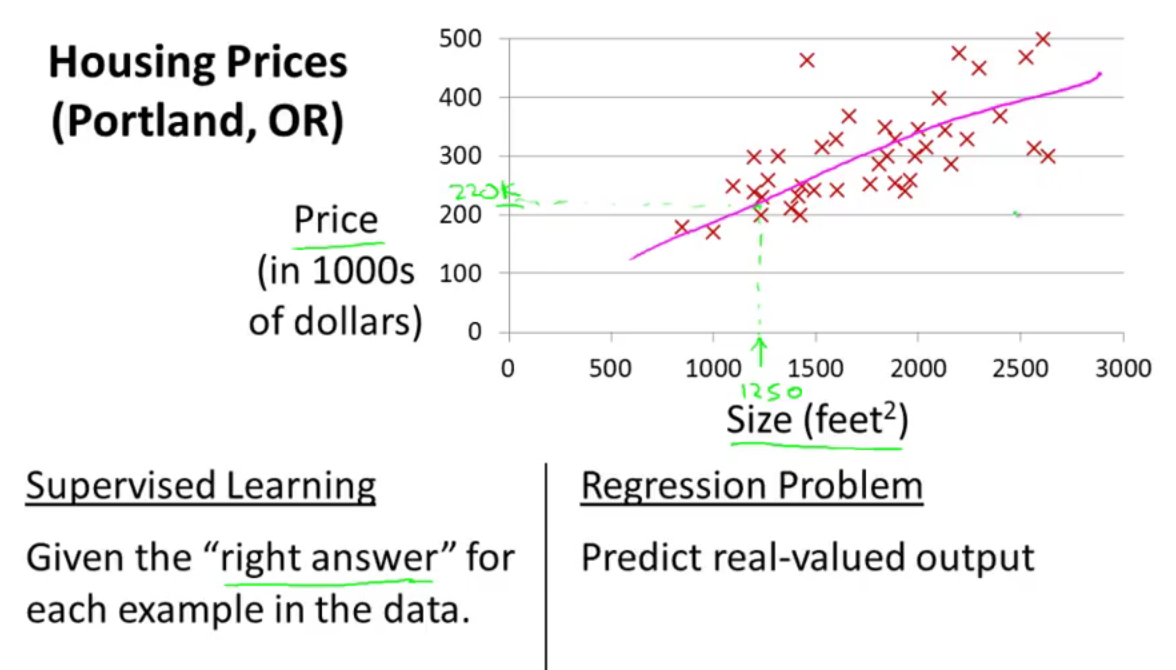
\includegraphics[scale=0.25]{img/MR1}
	\caption{Precios y tamaño de casas}
	\label{Fig:MR1}
\end{figure}
La notación que usaremos será la siguiente.
\begin{itemize}
	\item \textbf{m}: Número de datos de entrenamiento.
	\item \textbf{$x^{(i)}$}: Variables de entrada.
	\item \textbf{y}: Variables de salida
\end{itemize}
En nuestro ejemplo de las casas nuestras variables de entrada (\textbf{x}) serían el área de las casas. Las variables de salida son los precios de dichas casas.
\begin{table}
	\centering
	\begin{tabular}{c|c}
		Tamaño en $feet^2$ (x) & Precio en 1000 (y)\\
		\hline
		2104&460\\
		1416&232\\
		1534&315\\
		852&178
	\end{tabular}
\caption{Relación precio-área}
\label{Tab:TP}
\end{table}
Guiándonos en la tabla \ref{Tab:TP} diremos que\\$X^{(1)}=2104$ Cabe destacar que el 1 no es un exponente sino un índice.\\
Para obtener la función que mas se adapte a nuestros datos de entrenamiento tenemos que usar la función de hipótesis que se muestra en la ecuación \ref{Eq:Hipotesis} donde $\theta_0$ es el punto sobre el eje y donde pasa la recta y $\theta_1$ es la pendiente de la recta. si $\theta_0=0$ se dice que tenemos una regresión lineal con una variable, también es llamado regresión lineal univariable. 
\begin{equation}
	h_\theta(x)=\theta_0+\theta_1x
	\label{Eq:Hipotesis}
\end{equation}
\subsection{Función de costo}
Lo que se busca es que nuestra hipótesis sea la mejor, esto es que la distancia que hay de cada dato de entrenamiento y la recta que está definida por la función de hipótesis sea la menor posible. Cuando minimizamos estas distancias decimos que estamos minimizando el error. La función de costo nos regresa éste error, como su nombre lo indica nos está regresando el costo, por lo tanto lo que queremos hacer es minimizar esta función. La función de costo se indica en la ecuación \ref{Eq:FuncionCosto}. En este caso estamos trabajando con una sola variable por lo que $\theta_0=0$ y para este caso $(h_\theta(x^{(i)})$ es equivalente a $\theta_1x^{(i)}$. Nuestro objetivo siempre será minimizar la función de costo $J(\theta_0, \theta_1)$.
\begin{equation}
	J(\theta_0, \theta_1)=\frac{1}{2m}\sum_{i=0}^{m}(h_\theta(x^{(i)})-y^{(i)})^2
	\label{Eq:FuncionCosto}
\end{equation}
Vamos ver como se comporta la función de costo en a diferentes valores de $\theta_1$, para esto nos ayudaremos de la gráfica que se encuentra en la figura \ref{Fig:G1}.\\
Si $\theta_1=1$
\[
J(1)=\frac{1}{2m}(1*1-1)^2+(1*2-2)^2+(1*3-3)^2=0
\]
Nuestra hipótesis presenta un costo cero por lo que es una buena hipótesis y posiblemente la mejor.
\begin{figure}[hb]
	\centering
	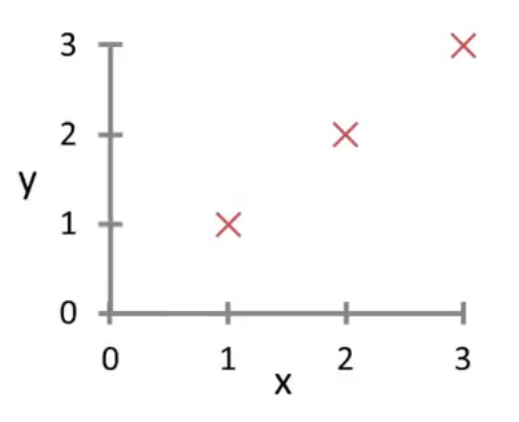
\includegraphics[scale=0.25]{img/Grafica}
	\caption{Gráfica x-y}
	\label{Fig:G1}
\end{figure}
Si hacemos $\theta_1=0.5$ tenemos:
\[
	J(0.5)=\frac{1}{2m}(0.5*1-1)^2+(0.5*2-2)^2+(0.5*3-3)^2=\frac{3.5}{6}\approx0.58
\]
Si hacemos $\theta_1=0$
\[
J(0)=\frac{1}{2m}(-1)^2+(-2)^2+(-3)^2=\frac{14}{6}
\]
Si seguimos dando valores a $\theta_1$ y graficamos los valores de la función de costo veremos que la función de costo es una paráblola donde el punto más bajo son las coordenadas (1,0).
\section{Parámetro de aprendizaje}
\subsection{Descenso de gradiente}
Como vimos anteriormente lo que buscamos en minimizar la función de costos, en esta sección veremos un algoritmo llamado el descenso de gradiente. Dicho algoritmo no sólo se utiliza en la regresión lineal sino en todo el aprendizaje automático. Con el descenso de gradiente podemos minimizar cualquier función no sólo la función de costos.\\Supongamos que tenemos una función $J(\theta_0,\theta_1)$ y queremos minimizarla, lo que hacemos es darle un valor aleatorio a $\theta_0$ y $\theta_1$, lo que haremos es cambiar estos valores de manera que que en cada cambio que hagamos $J(\theta_0,\theta_1)$ se cada vez menor.\\\\Supongamos que la superficie que se muestra en la figura \ref{Fig:GD1} es la representación gráfica de una función de costos dada una función de hipótesis y aleatoriamente elegimos valores para $\theta_0$ y $\theta_1$ éste punto se muestra en la imagen como la primera cruz negra que esta en el punto más alto. Imaginemos que tu estas parado en una colina que se representa por la función $J(\theta_0,\theta_1)$ vista en la imagen, y tu posición es el punto $\theta_0$ y $\theta_1$, ahora lo que quieres es dar un paso de tal forma que vayas hacia abajo, das este paso y después vuelves a ver en que dirección debes dar el siguiente paso para ir cada vez más abajo, estos pasos se representan en la figura con las estrellas negras.\\ Como podemos ver después de una serie de repeticiones llegamos al punto más bajo de toda la función, los valores $\theta_0$ y $\theta_1$ son valores bastante aceptables para trabajar nuestra hipótesis. el algoritmo de descenso de gradiente se muestra en la ecuación \ref{Eq:DG} este algoritmo se tiene que repetir hasta que converga.
\begin{figure}[h]
	\centering
	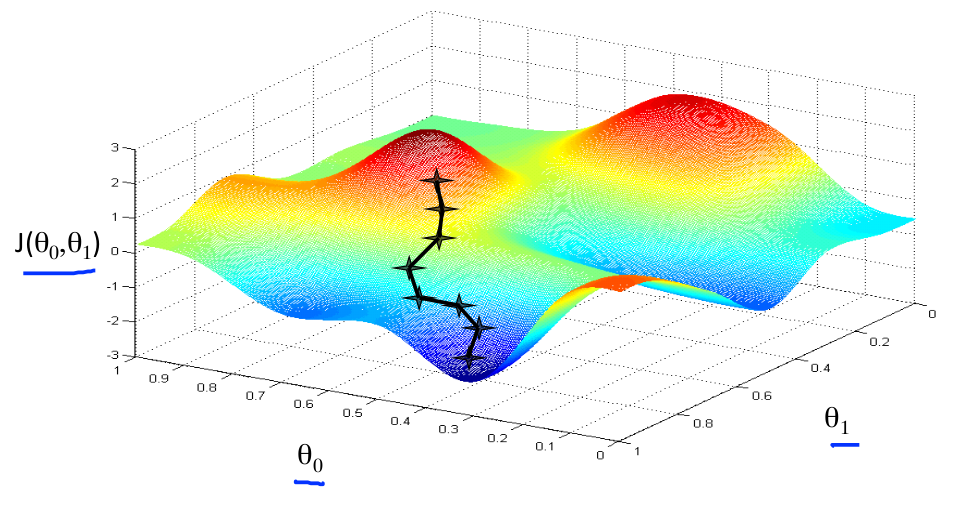
\includegraphics[scale=0.5]{img/GD1}
	\caption{Minimización de $J(\theta_0,\theta_1)$}
	\label{Fig:GD1}	
\end{figure}
\begin{equation}
	\theta_j := \theta_j -\alpha\frac{\partial}{\partial\theta_j}J(\theta_0,\theta_1)\qquad Para\quad j=0\quad y\quad j=1
	\label{Eq:DG}
\end{equation}
Lo que le estamos diciendo es que con cada iteración el valor de $\theta_j$ se tiene que actualizar a un nuevo valor que tiene que ser menor al anterior.\\$\alpha$ es el índice de aprendizaje y lo que hace es controlar qué tan grande el un paso que estamos dando con el gradiente de descenso, si $\alpha$ es muy grande estamos dando pasos muy grandes hacia abajo, si $\alpha$ es pequeño estaremos dando pasos muy pequeños. Uno de nuestros objetivos es encontrar el mejor valor de $\alpha$ ya que al dar pasos muy grandes puede que oscile todo el tiempo entre valores bajos y altos entrando en un bucle infinito y puede que no converga. Si $\alpha$ da pasos muy pequeños tardará demasiado nuestro algoritmo en encontrar una solución aparte de consumir muchos recursos. Mas adelante veremos como encontrar el mejor valor para $\alpha$.\\Algo que tenemos que tomar en cuenta para este algoritmo es que tiene que haber una actualización simultanea entre los términos $\theta_0$ y $\theta_1$ como se muestra en las ecuaciones desde la \ref{Eq:A1} a \ref{Eq:A4}.
\begin{align}
	temp_0&:= \theta_0 -\alpha\frac{\partial}{\partial\theta_0}J(\theta_0,\theta_1)\label{Eq:A1}\\
	temp_1&:= \theta_1 -\alpha\frac{\partial}{\partial\theta_1}J(\theta_0,\theta_1)\label{Eq:A2}\\
	\theta_0&:=temp_0\label{Eq:A3}\\
	\theta_1&:=temp_1\label{Eq:A4}
\end{align}
Lo que vamos a hacer a continuación es usar el gradiente de descenso para minimizar la función de costo, para esto nos vamos a centrar en las derivadas parciales de dicha función.
\begin{equation}
	\frac{\partial}{\partial\theta_j}J(\theta_0, \theta_1)=\frac{\partial}{\partial\theta_j}\frac{1}{2m}\sum_{i=0}^{m}(h_\theta(x^{(i)})-y^{(i)})^2=\frac{\partial}{\partial\theta_j}\frac{1}{2m}\sum_{i=0}^{m}(\theta_0+\theta_1x^{(i)}-y^{(i)})^2
	\label{Eq:GD2}
\end{equation}
A partir de la ecuación \ref{Eq:GD2} podemos escribir las derivadas parciales tanto para $\theta_0$ como para $\theta_1$ como se muestra a continuación.
\begin{align}
	\frac{\partial}{\partial\theta_0}J(\theta_0, \theta_1)=&\frac{1}{m}\sum_{i=0}^{m}(h_\theta(x^{(i)})-y^{(i)})\label{Eq:AI1}\\
	\frac{\partial}{\partial\theta_1}J(\theta_0, \theta_1)=&\frac{1}{m}\sum_{i=0}^{m}(h_\theta(x^{(i)})-y^{(i)})x^{(i)}\label{Eq:AI2}
\end{align}
Ahora lo que hacemos es sustituir las ecuaciones \ref{Eq:AI1} y \ref{Eq:AI2} en \ref{Eq:A1} y \ref{Eq:A2} respectivamente. De igual forma tenemos que actualizar $\theta_0$ y $\theta_1$ hasta que convergan.
\begin{align}
	\theta_0&:=\theta_0-\alpha\frac{1}{m}\sum_{i=0}^{m}(h_\theta(x^{(i)})-y^{(i)})\label{Eq:AI2-1}\\
	\theta_1&:=\theta_1-\alpha\frac{1}{m}\sum_{i=0}^{m}(h_\theta(x^{(i)})-y^{(i)})x_1^{(i)}\label{Eq:AI2-2}\\
\end{align}
\begin{wrapfigure}[16]{l}{0.58\textwidth}
	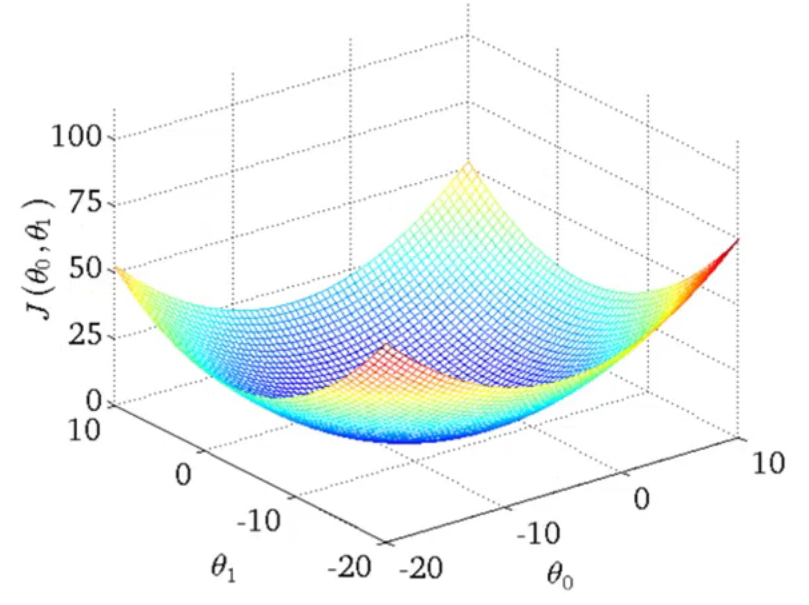
\includegraphics[scale=0.31]{img/CF-RL}
	\caption{Función de costo para una regresión lineal}
	\label{Fig:CFRL}
\end{wrapfigure}
La función de costos para la regresión lineal siempre será convexa y en forma de arco tal y como se ve en la figura \ref{Fig:CFRL}.\\
Cuando obtenemos el mínimo de la función siempre será un mínimo global ya que es el único punto más bajo que tiene, a diferencia de la función que se muestra en la figura \ref{Fig:GD1} que también poseé mínimos locales.\\Entonces si encontramos los valores $\theta_0$ y $\theta_1$ del punto más bajo de la función $j(\theta_0, \theta_1)$ y sustituimos dichos valores en la función de hipótesis diremos que dicha función puede predecir un valor con una exactitud aceptable. 
\chapter{Regresión lineal con múltiples variables}
\section{Múltiples características}
Hasta este punto habíamos puesto como ejemplo predecir el precio de una casa dado su tamaño, que pasaría si queremos predecir el precio de una casa pero no sólo tenemos su tamaño como característica si también contamos con otras como el numero de habitaciones, pisos, años que tiene la casa de ser construida, etc. Dichas características se encuentran en la tabla \ref{Tab:Multi}.
\begin{table}[h]
		\begin{tabular}{|c|c|c|c||c|}
			\hline
			Tamaño ($feet^2$) & Número de habitaciones & Número de pisos&Años de la casa&Precio(\$1000)\\
			\hline
			\hline
			2104&5&1&45&460\\
			1416&3&2&40&232\\
			1534&3&2&30&315\\
			852&2&1&36&4178\\
			\dots&\dots&\dots&\dots&\dots\\		
			\hline	
		\end{tabular}
	\caption{Múltiples características}
	\label{Tab:Multi}
\end{table}
\\Ahora vamos a hablar sobre la notación que usaremos. El tamaño sera nuestra variable $x_1$ el número de habitaciones será $x_2$ y así sucesivamente, el valor del precio será nuestra variable $y$.\\\\
\textbf{\textit{$n$}}: Número de características.\\
\textbf{\textit{$x^{i}$}}: Características del $i$-ésimo dato de entrenamiento (Filas).\\
\textbf{\textit{$x^{i}_j$}}: Valor de la característica $j$ en el $i$-ésimo dato de entrenamiento.\\\\
En el ejemplo mostrado en la tabla $n=4$ ya que tenemos 4 características, $m=4$ ya que tenemos 4 datos de entrenamiento. El valor que corresponde a $ x_3^{(2)}=2$ y $x^{(2)}$ se representa como una matriz de $4X1$ cuyos valores son 1416, 3, 2, 40.
\[x^{(2)}=\left[
\begin{array}{c}
	1416\\3\\2\\40
\end{array}
\right]
\]
Al trabajar con mas características tenemos que cambiar nuestra función de hipótesis como se muestra en la ecuación \ref{Eq:Hip2}.
\begin{equation}
	h_\theta(x)=\theta_0+\theta_1x_1+\theta_2x_2+\dots+\theta_nx_n
	\label{Eq:Hip2}
\end{equation}
En nuestro ejemplo $\theta_0$ es el precio base de la casa, $\theta_1$ es el precio por $feet^2$, $\theta_2$ es el precio por una habitación, $\theta_3$ es el precio por un piso y $\theta_4$ es el precio por cada año de la casa, podemos considerar la casa pierde su valor en función de los años por lo tanto $\theta_4$ sería un valor negativo.\\
$x_1$ es el número de $feet^2$ que tiene la casa, $x_2$ es el número de habitaciones, $x_3$ es el número de pisos que tiene la casa, $x_4$ son los años que tiene la casa. Por convención $x_0^{(i)}=1$. Lo que haremos a continuación será vectorizar las variables $x$ y $\theta$ como se muestra en la ecuación \ref{Eq:Vecto}.
\begin{equation}
x=\left[
\begin{array}{c}
	x_0\\x_1\\x_2\\\vdots\\x_n
\end{array}
\right]\in \mathbb{R}^{n+1}\qquad
\theta=\left[
\begin{array}{c}
\theta_0\\\theta_1\\\theta_2\\\vdots\\\theta_n
\end{array}
\right]\in \mathbb{R}^{n+1}\qquad
\theta^T=\left[
\begin{array}{ccccc}
\theta_0&\theta_1&\theta_2&\dots&\theta_n
\end{array}
\right]
\label{Eq:Vecto}
\end{equation}
Entonces tenemos que:
\begin{equation}
h_\theta(x)=\theta_0x_0+\theta_1x_1+\theta_2x_2+\dots+\theta_nx_n=\theta^Tx
\label{Eq:HipVecto}
\end{equation}
Lo que tenemos que hacer es de igual forma como en el caso de una variable, actualizar los valores de $\theta$ con un algoritmo iterativo hasta que estos convergan.
\begin{align}
\theta_0&:=\theta_0-\alpha\frac{1}{m}\sum_{i=0}^{m}(h_\theta(x^{(i)})-y^{(i)})x_0^{(i)}\label{Eq:AI3-1}\\
\theta_1&:=\theta_1-\alpha\frac{1}{m}\sum_{i=0}^{m}(h_\theta(x^{(i)})-y^{(i)})x_1^{(i)}\label{Eq:AI3-2}\\
\theta_2&:=\theta_2-\alpha\frac{1}{m}\sum_{i=0}^{m}(h_\theta(x^{(i)})-y^{(i)})x_2^{(i)}\label{Eq:AI3-3}\\
\dots\notag
\end{align}
Visto de otra forma nuestro algoritmo para múltiples variables queda resumido en la ecuación \ref{Eq:AI3-Resumido}
\begin{equation}
\theta_j:=\theta_j-\alpha\frac{1}{m}\sum_{i=0}^{m}(h_\theta(x^{(i)})-y^{(i)})x_j^{(i)} \qquad Para\quad j:=0\dots n
\label{Eq:AI3-Resumido}
\end{equation}
\section{Escalamiento de características}
Al trabajar con múltiples características tenemos que tomar en cuenta el rango de valores que estas toman, por ejemplo tenemos una característica que es el tamaño de la casa cuyos valores oscilan entre 0-2000 y tenemos otra característica que es el número de habitaciones cuyos valores oscilan entre 1-5.\\\\Al ejecutar el gradiente de descenso puede oscilar dando pasos muy grandes o muy pequeños, este comportamiento se sale de nuestro control y puede que el valor nunca converga.\\Lo que hacemos para evitar esto es escalar los valores de nuestras características, es decir que todas tomen un rango similar idealmente entre $-1\underline{<} x_i \underline{<}1$ es aceptable un rango un poco más grande o más pequeño. \\\\Por ejemplo que los rangos de valores de nuestras características se encuentren en $0\underline{<}x_1\underline{<}3$ o $-2\underline{<}x_2\underline{<}0.5$, lo que no está permitido es tomar rangos muy grandes o muy pequeños como $-100\underline{<}x_3\underline{<}100$ o $-0.0001\underline{<}x_4\underline{<}0.0001$.\\La ecuación que usaremos para hacer este escalamiento se muestra en la ecuación \ref{Eq:Esc}.
\begin{equation}
	x_i:=\frac{x_i-\mu_i}{s_i}
	\label{Eq:Esc}
\end{equation}
Donde:\\$x_i$ es la característica que queremos escalar.\\$\mu_i$ es el promedio de los valores de dicha característica.\\
$s_i$ Es el rango de valores (Valor maximo - Valor mínimo).\\\\Por ejemplo si queremos escalar la característica de número de habitaciones haríamos lo siguiente.
\[
x_2=\frac{\#Habitaciones-2}{5}
\]
\end{document}
